
\section{Results}

\subsection{Taxonomic profiles show evidence of continual microbial exchange}



\paragraph{Novel taxa in TW match environmental and commensal microbiomes}

\begin{figure}
  \begin{center}
    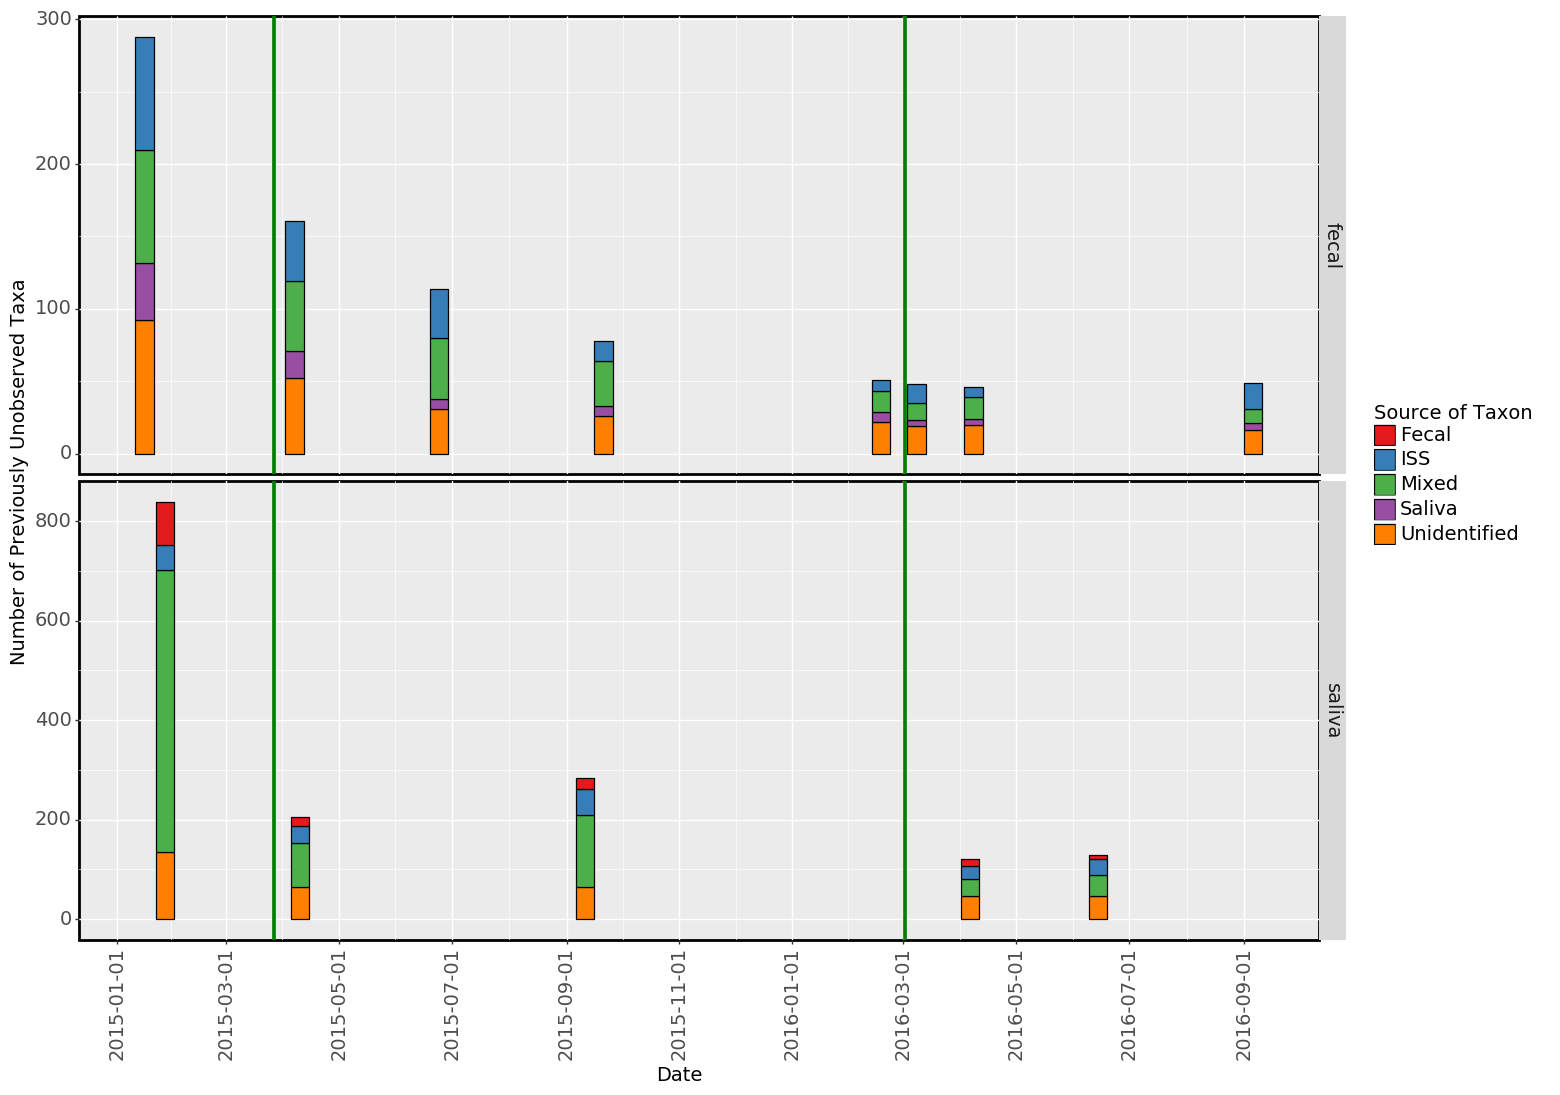
\includegraphics[width=0.99\textwidth]{figs/twins_taxa_sources.png}
%	\vspace{-20pt}
	\caption{\small{
	    This plot shows the number of taxa at each time point that were not observed at any previous timepoint for fecal and saliva samples from TW. The colors indicate the likely source of the new taxon if it was found previously in the saliva (for fecal samples, vice versa for saliva samples), the ISS, both (Mixed), or neither.
	}}
    \label{fig:taxasource}
  \end{center}
%  \vspace{-20pt}
 % \vspace{1pt}
\end{figure}

\begin{figure}
  \begin{center}
    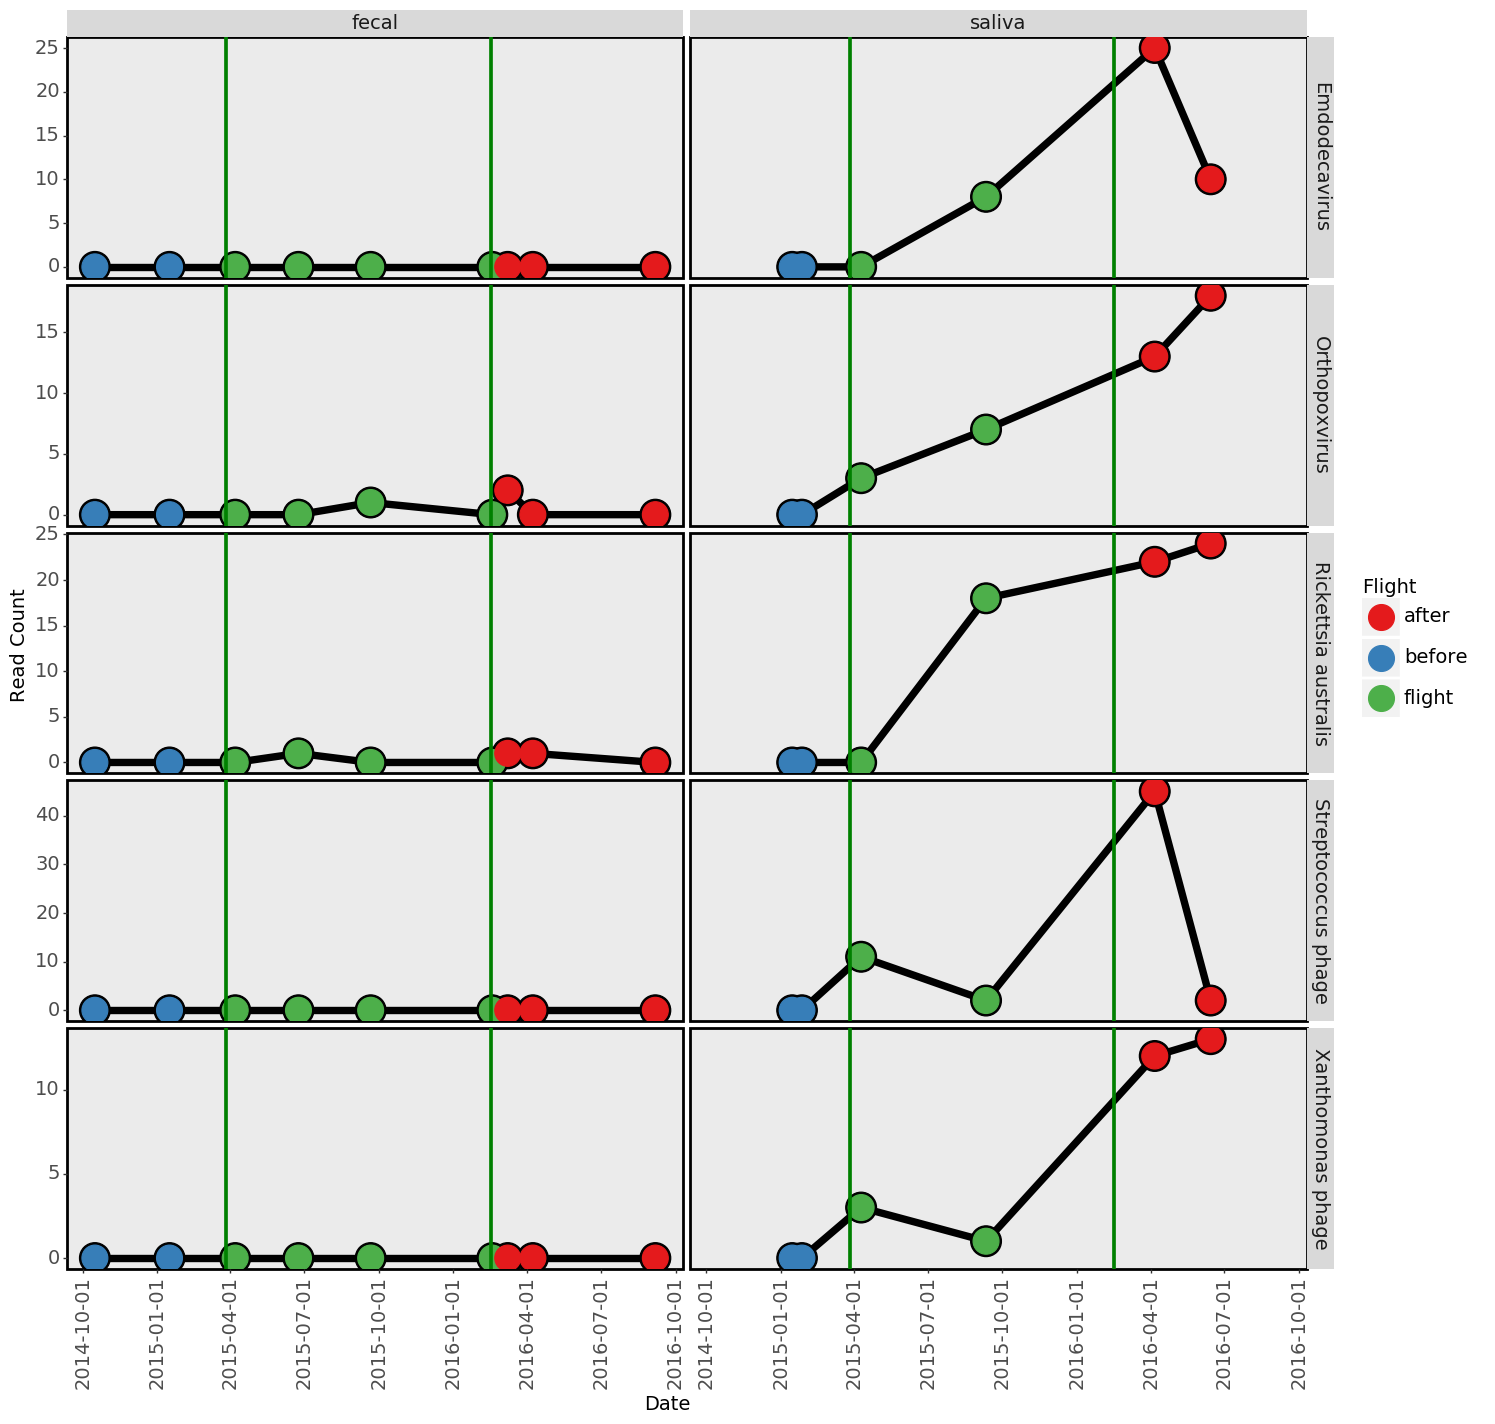
\includegraphics[width=0.99\textwidth]{figs/tw_flight_taxa.png}
%	\vspace{-20pt}
	\caption{\small{
	    Total number of reads observed in TW for different taxa at different time points. Green vertical bars indicate the start and end of flight.
	}}
    \label{fig:flighttaxa}
  \end{center}
%  \vspace{-20pt}
 % \vspace{1pt}
\end{figure}

Repeated sampling of a microbiome will identify taxa not observed in previous samples from the same site. This can be due either to technical or biological variation. The time series of samples taken from TW and HR match this trend. Importantly, for these time series many of the newly observed taxa in each time series were observed in samples from other sites. These samples were either from the ISS or from other body sites in TW. We identified possible sources for different newly observed taxa in each time series. For fecal samples from TW we segmented the previously unobserved taxa from each sample into four groups: taxa observed in any saliva sample taken before the given fecal samples, taxa observed in ISS samples but not observed in saliva, taxa observed in both ISS and saliva samples, and taxa that were not observed in either the ISS or the saliva. The same process was repeated for saliva samples but swapping fecal and saliva in the hierarchy.

The number of previously unobserved taxa assigned to each group is shown in Figure \ref{fig:taxasource}. An analagous plot for HR can be found at Figure \ref{fig:hrtaxasource}. Each sample contains a number of unobserved taxa that matched taxa from saliva/feces or the ISS. Taxa that match taxa in the ISS can be found in TW before flight and in HR. It is unlikely these taxa are actually from the ISS (though admittedly both TW and HR had been to the ISS on previous occasions) so it is likely that these are common environmental taxa found regularly on earth. However, the fraction of taxa that match ISS taxa is increased for peri-flight samples from TW compared to other samples. On average 56\% of taxa in peri-flight samples from TW match taxa from the ISS (either ISS or Mixed) compared to 51\% for other samples. Due to the small sample size this result does not achieve significance with a p value of just 0.21. 

\begin{table}[]
\centering
\caption{This table gives the average overlap between emergent taxa in fecal and saliva microbiomes and microbiomes in other sites.}
\label{tbl:sourcepercents}
\begin{tabular}{lrr}
\toprule
Commensal Type &      Fecal &     Saliva \\
\midrule
Sites Where Taxa Originated     &            &            \\
%\midrule
Fecal Only       &  n/a &   8.7  \\
Saliva Only      &  10.2 &  n/a  \\
ISS Only        &  24.5 &  17.6 \\
Both ISS \& Saliva/Fecal        &  29.9 &  44.6 \\
Taxa not identified in another site &  35.5 &  29.1 \\
\bottomrule
\end{tabular}
\end{table}

On its own these data do not definitively establish transfer between the ISS environment and TW. Rather these let us estimate a boundary for the fraction of taxa that could be transferred from different sources. The fraction of taxa that matched different environments are listed in Table \ref{tbl:sourcepercents}. For both saliva and fecal microbiomes the large majority of taxa at each time point had already been observed in a previous sample from that site.  

A small number of taxa were never observed in any pre-flight sample from any body site but were observed in peri and post-flight samples. We filtered for taxa that had no reads observed in pre-flight samples and had at least ten reads in at least two peri or post-flight samples. These taxa were further filtered for taxa that were observed in at least two ISS samples. The resulting list included five taxa: two viral genera, two viral species (both phage), and one bacterial species: Rickettsia australis (Figure \ref{fig:flighttaxa}). Given the generally low abundance of these taxa we cannot definitively rule out that they were present at an undetectable low threshold pre-flight.


\paragraph{Emergence of novel taxa in gut microbiomes exceeds repeated sampling} 

\begin{figure}
  \begin{center}
    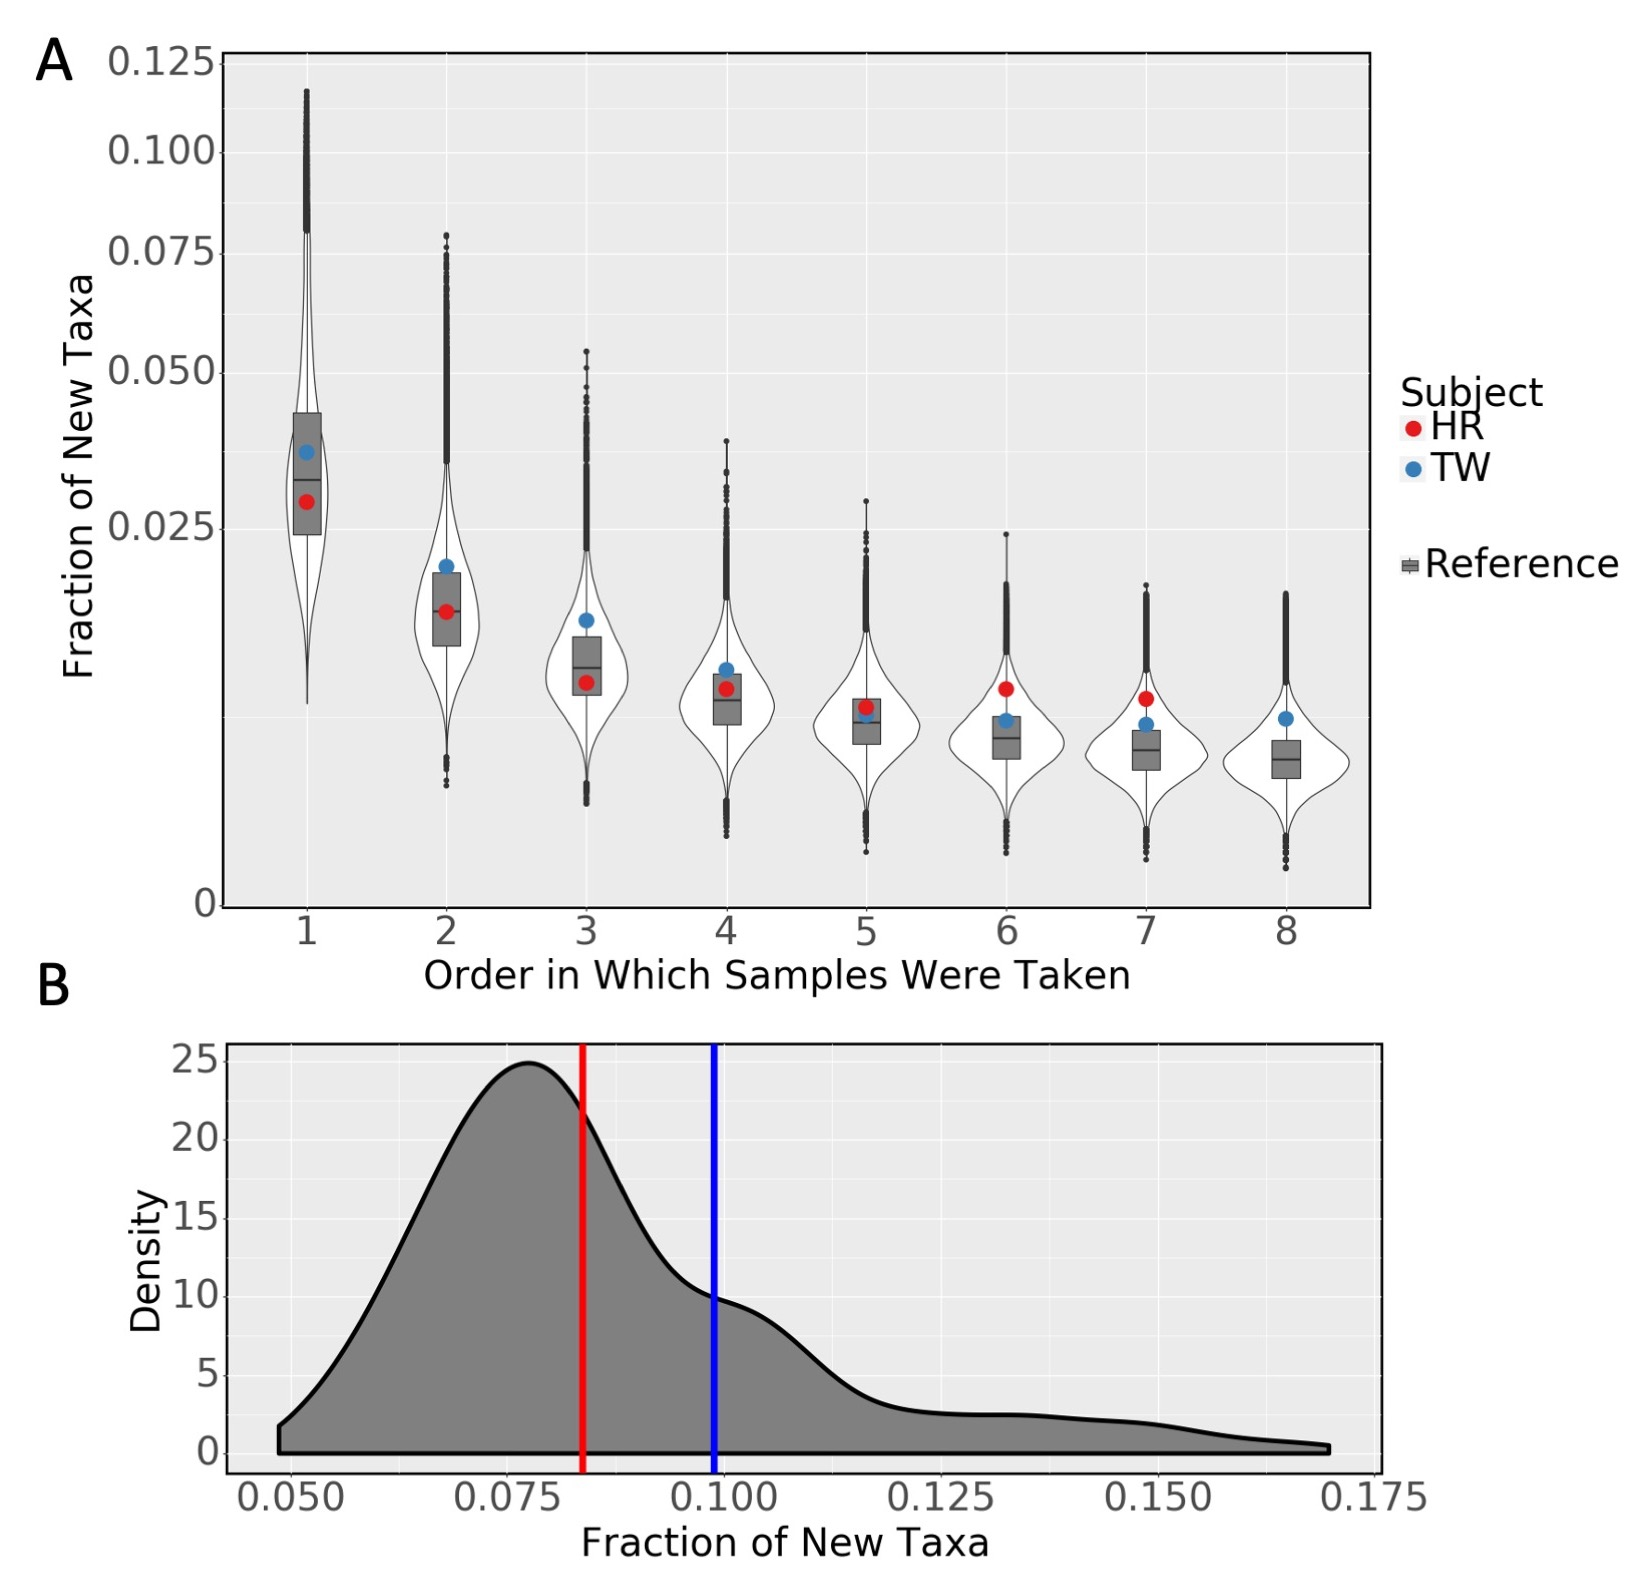
\includegraphics[width=0.99\textwidth]{figs/taxa_repeated_sampling.jpg}
%	\vspace{-20pt}
	\caption{\small{
	    A) The number of new taxa observed in TW and HR are higher than repeated resampling of the same fecal sample. The y-axis gives the number of new taxa at each time point (not observed at any previous time point) divided by the number of taxa in the first sample. The first time point is omitted from the plot because it is always 1 by construction. The x-axis gives the order of each sample (arbitrary for random subsample). Boxplots show the distribution of random subsamples. Colored points are the actual time series.
	    B) The number of unique taxa observed after the first time point divided by the number of taxa at the first time point. Same legend as (A)
	}}
    \label{fig:taxarepeated}
  \end{center}
%  \vspace{-20pt}
 % \vspace{1pt}
\end{figure}

In most cases taking multiple samples of the same microbiome will identify taxa that were not observed in previous samples even if the microbiome has not changed. This is largely because repeated sampling can identify low abundance species which were dropped out of previous samples and because different sample preparation techniques can yield different sets of taxa. A series of samples taken from a microbiome that is exchanging taxa with an external environment will have an additional source of new taxa. These taxa would not be identified in earlier samples because they were not present. We investigated whether time series from TW and HR would identify more new taxa than repeated assays on an unchanging sample.

We compared time series of fecal microbiome samples from TW and HR to 243 repeated samples (technical replicates) taken from a single fecal source sample. These 243 samples were processed with different lysis techniques which could lead to different taxonomic profiles \citep{Sasada2020}. We took 100,000 random subsets of 9 (the same number of samples in the time series for TW and HR) samples from the set of 243. WE treated each set of 9 samples as an ordered time series. We counted the number of taxa in each sample that had not been observed in any previous sample for each subset and normalized the number of taxa by the total number of taxa in the first sample. We repeated the same process for the time series from TW and HR using the actual order in which the samples were taken.

We compared the number of new taxa in TW and HR to the random subsets (Figure \ref{fig:taxarepeated}). We counted the number of random subsets that had more taxa at each time point than were identified in TW and HR. The time series for HR had more taxa than 99,971 (p 2.9e-4) random subsets, TW had more taxa than 99,990 (p 1e-4) subsets. This result shows that the time series for TW and HR both consistently had more taxa than would be expected from  resampling an unchanged fecal sample. This implies that the microbiomes from TW and HR are dynamic continually producing previously unobserved taxa.

We note that many of the 100,000 subsets had more newly observed taxa at some (but not all) of the time points. This is particularly true for early time points and is consistent with the idea that different taxa can be identified by different sample preparation techniques. Importantly the number of new taxa that were observed in subsets dropped off quickly for later time points as the subsets reached saturation. Subsets generally showed an adversarial selection where many new taxa at one time point would lead to fewer new taxa at later time points. The 243 fecal replicates had similar read counts to the time series from HR and TW. Fecal samples from the twins had about 56M classified reads on average compared to about 44M for the fecal replicates.

\paragraph{Evidence of higher transfer rates on board the ISS}

We calculated taxonomic diversity using Shannon's entropy for species profiles of each sample (Figure \ref{fig:taxadiv}). For both fecal and saliva samples from TW the highest diversity was observed during flight. This was not observed for HR. However, given the small number of samples it is unlikely that samples taken during flight could be shown to be significantly more diverse.

% In most settings repeated sampling of the same microbiome will yield species which were not identified in previous sampling. This can be due, primarily, to two factors: natural variation and evolution of a microbiome or experimental error and dropout of species. The latter is likely to be a consistent error given consistent experimental setting while the former can vary based on external conditions.  

 For time series of buccal, fecal, and saliva samples from TW and HR. We identified species which had not previously been observed in any sample. The number of new species discovered in each sample varied by time point. Later samples generally had fewer new species (as expected) though with substantial variation.

We identified a significant increase in the number of previously unobserved taxa for samples taken from TW during flight (Figure \ref{fig:taxaflux}). To demonstrate this we performed a permutation test. We started by establishing the number of previously unobserved species found at each time point in the actual data from TW. We then randomly shuffled and relabeled these samples and counted species again. We noted if the number of species observed 'during flight' in the shuffled data was higher than the real data and repeated the shuffling 10,000 times (Caveat: we only had three samples for the buccal microbiome and all 6 permutations were tried). For the fecal microbiome the actual number of observed taxa was higher than the shuffled data in 96.7\% of cases, for saliva 98.2\% of cases and for buccal the observed was higher than all other permutations. Repeating the same procedure on data from HR ('flight' status was arbitrarily assigned to the second, third, and fourth samples)  we observed 45.9\% for feces 98.2\% for saliva, and 80.1\% for buccal (more buccal samples were available for HR). Results were similar when the above procedure was repeated only with taxa found in ISS environmental samples.

\subsection{Strain level variation confirms microbial transfer}

\begin{table}[]
\centering
\caption{Size of regions that may have been transferred in kilobases. Gut-Saliva transfer means that a region was found in either the gut or saliva microbiome pre-flight, then found in the other during-flight. Environment transfer means a region was not found in either fecal or saliva microbiomes from TW pre-flight but was found during flight and was also present in the ISS.}
\label{tbl:covcounts}
\begin{tabular}{lrrr}
\toprule
{} &  Pre-flight &  Gut-Saliva transfer &  Environment transfer \\
\midrule
Bifidobacterium pseudocatenulatum &                  243.9 &                 92.4 &                  85.2 \\
Brevibacterium siliguriense       &                   18.7 &                  2.6 &                   3.1 \\
Gordonibacter urolithinfaciens    &                   37.8 &                 12.9 &                  21.2 \\
Bacillus albus                    &                   87.6 &                  7.0 &                  14.1 \\
Gluconobacter albidus             &                   10.2 &                  2.5 &                   1.3 \\
Fusobacterium necrophorum         &                   86.4 &                 18.0 &                  56.8 \\
Geobacillus stearothermophilus    &                   73.5 &                 13.7 &                  13.8 \\
Bifidobacterium catenulatum       &                  258.8 &                 17.5 &                  40.3 \\
Streptococcus viridans            &                 2319.6 &                 92.9 &                 221.8 \\
Vibrio alginolyticus              &                  211.0 &                 10.6 &                  89.7 \\
Staphylococcus sciuri             &                  179.0 &                 19.4 &                  37.4 \\
Pectobacterium parmentieri        &                  269.0 &                 22.7 &                  56.7 \\
Campylobacter lari                &                   42.0 &                  8.7 &                  18.1 \\
Atlantibacter hermannii           &                   66.4 &                 15.7 &                  30.6 \\
Bacillus tequilensis              &                   57.4 &                  6.0 &                   8.7 \\
Achromobacter ruhlandii           &                   49.8 &                 13.6 &                  11.7 \\
Serratia proteamaculans           &                   70.0 &                 11.2 &                   6.7 \\
Leptotrichia hongkongensis        &                  115.2 &                  0.7 &                  21.5 \\
Exiguobacterium antarcticum       &                   21.5 &                  4.4 &                   6.2 \\
Anoxybacillus amylolyticus        &                   11.5 &                  2.2 &                   2.3 \\
Kosakonia sacchari                &                   65.4 &                 16.0 &                  30.8 \\
Yersinia canariae                 &                   18.2 &                  8.2 &                   7.7 \\
Providencia heimbachae            &                   76.0 &                 12.1 &                   6.5 \\
Spirochaeta perfilievii           &                    2.7 &                  0.4 &                   0.7 \\
Cronobacter condimenti            &                   15.2 &                  8.5 &                  18.8 \\
Brenneria rubrifaciens            &                   13.2 &                  5.7 &                   7.3 \\
Staphylococcus simiae             &                   20.8 &                  1.5 &                   6.2 \\
\bottomrule
\end{tabular}
\end{table}

\paragraph{Novel genome regions in flight found in environmental and commensal microbiomes}

We selected a set of species that were significantly more abundant during and after flight in TW than they were before flight. We then mapped reads to reference genomes from these taxa and observed the results. We looked at the coverage of reference genomes at each stage of flight (concatenating samples from the same stage) and in the ISS.  Example coverage plots for \textit{Fusobacterium necrophorum}  and \textit{Serratia proteamaculans} are shown in Figure \ref{fig:fnecro} and Figure \ref{fig:sprota} respectively.

For each species we grouped regions into three categories: regions which were covered before flight, regions that were covered before flight in either gut or saliva samples but not observed in the other until flight, and regions that were not observed in either gut or saliva samples until flight but were found in the environment. The total size of these regions for all tested taxa are listed in  Table \ref{tbl:covcounts}.

For the selected taxa on average environmental transfer regions were 32.2\% of the size of pre-flight regions. While gut-saliva transfers were 19.9\%. There was wide variation in these numbers for individual taxa. The taxa with the (proportionally) largest transferred regions, \textit{Cronobacter condimenti}, had 55.9\% gut-saliva transfer and 123.7\% environmental transfer. 

The presence of (in some taxa) large genomic regions that were not covered until flight strongly suggests that individual species are undergoing flux with new strains and genes migrating into commensal microbiomes. These regions match regions found in the ISS or in other commensal microbiomes further suggesting a source for the new regions.


\paragraph{Microbial SNPs match environmental and commensal microbiomes}



\begin{figure}
  \begin{center}
    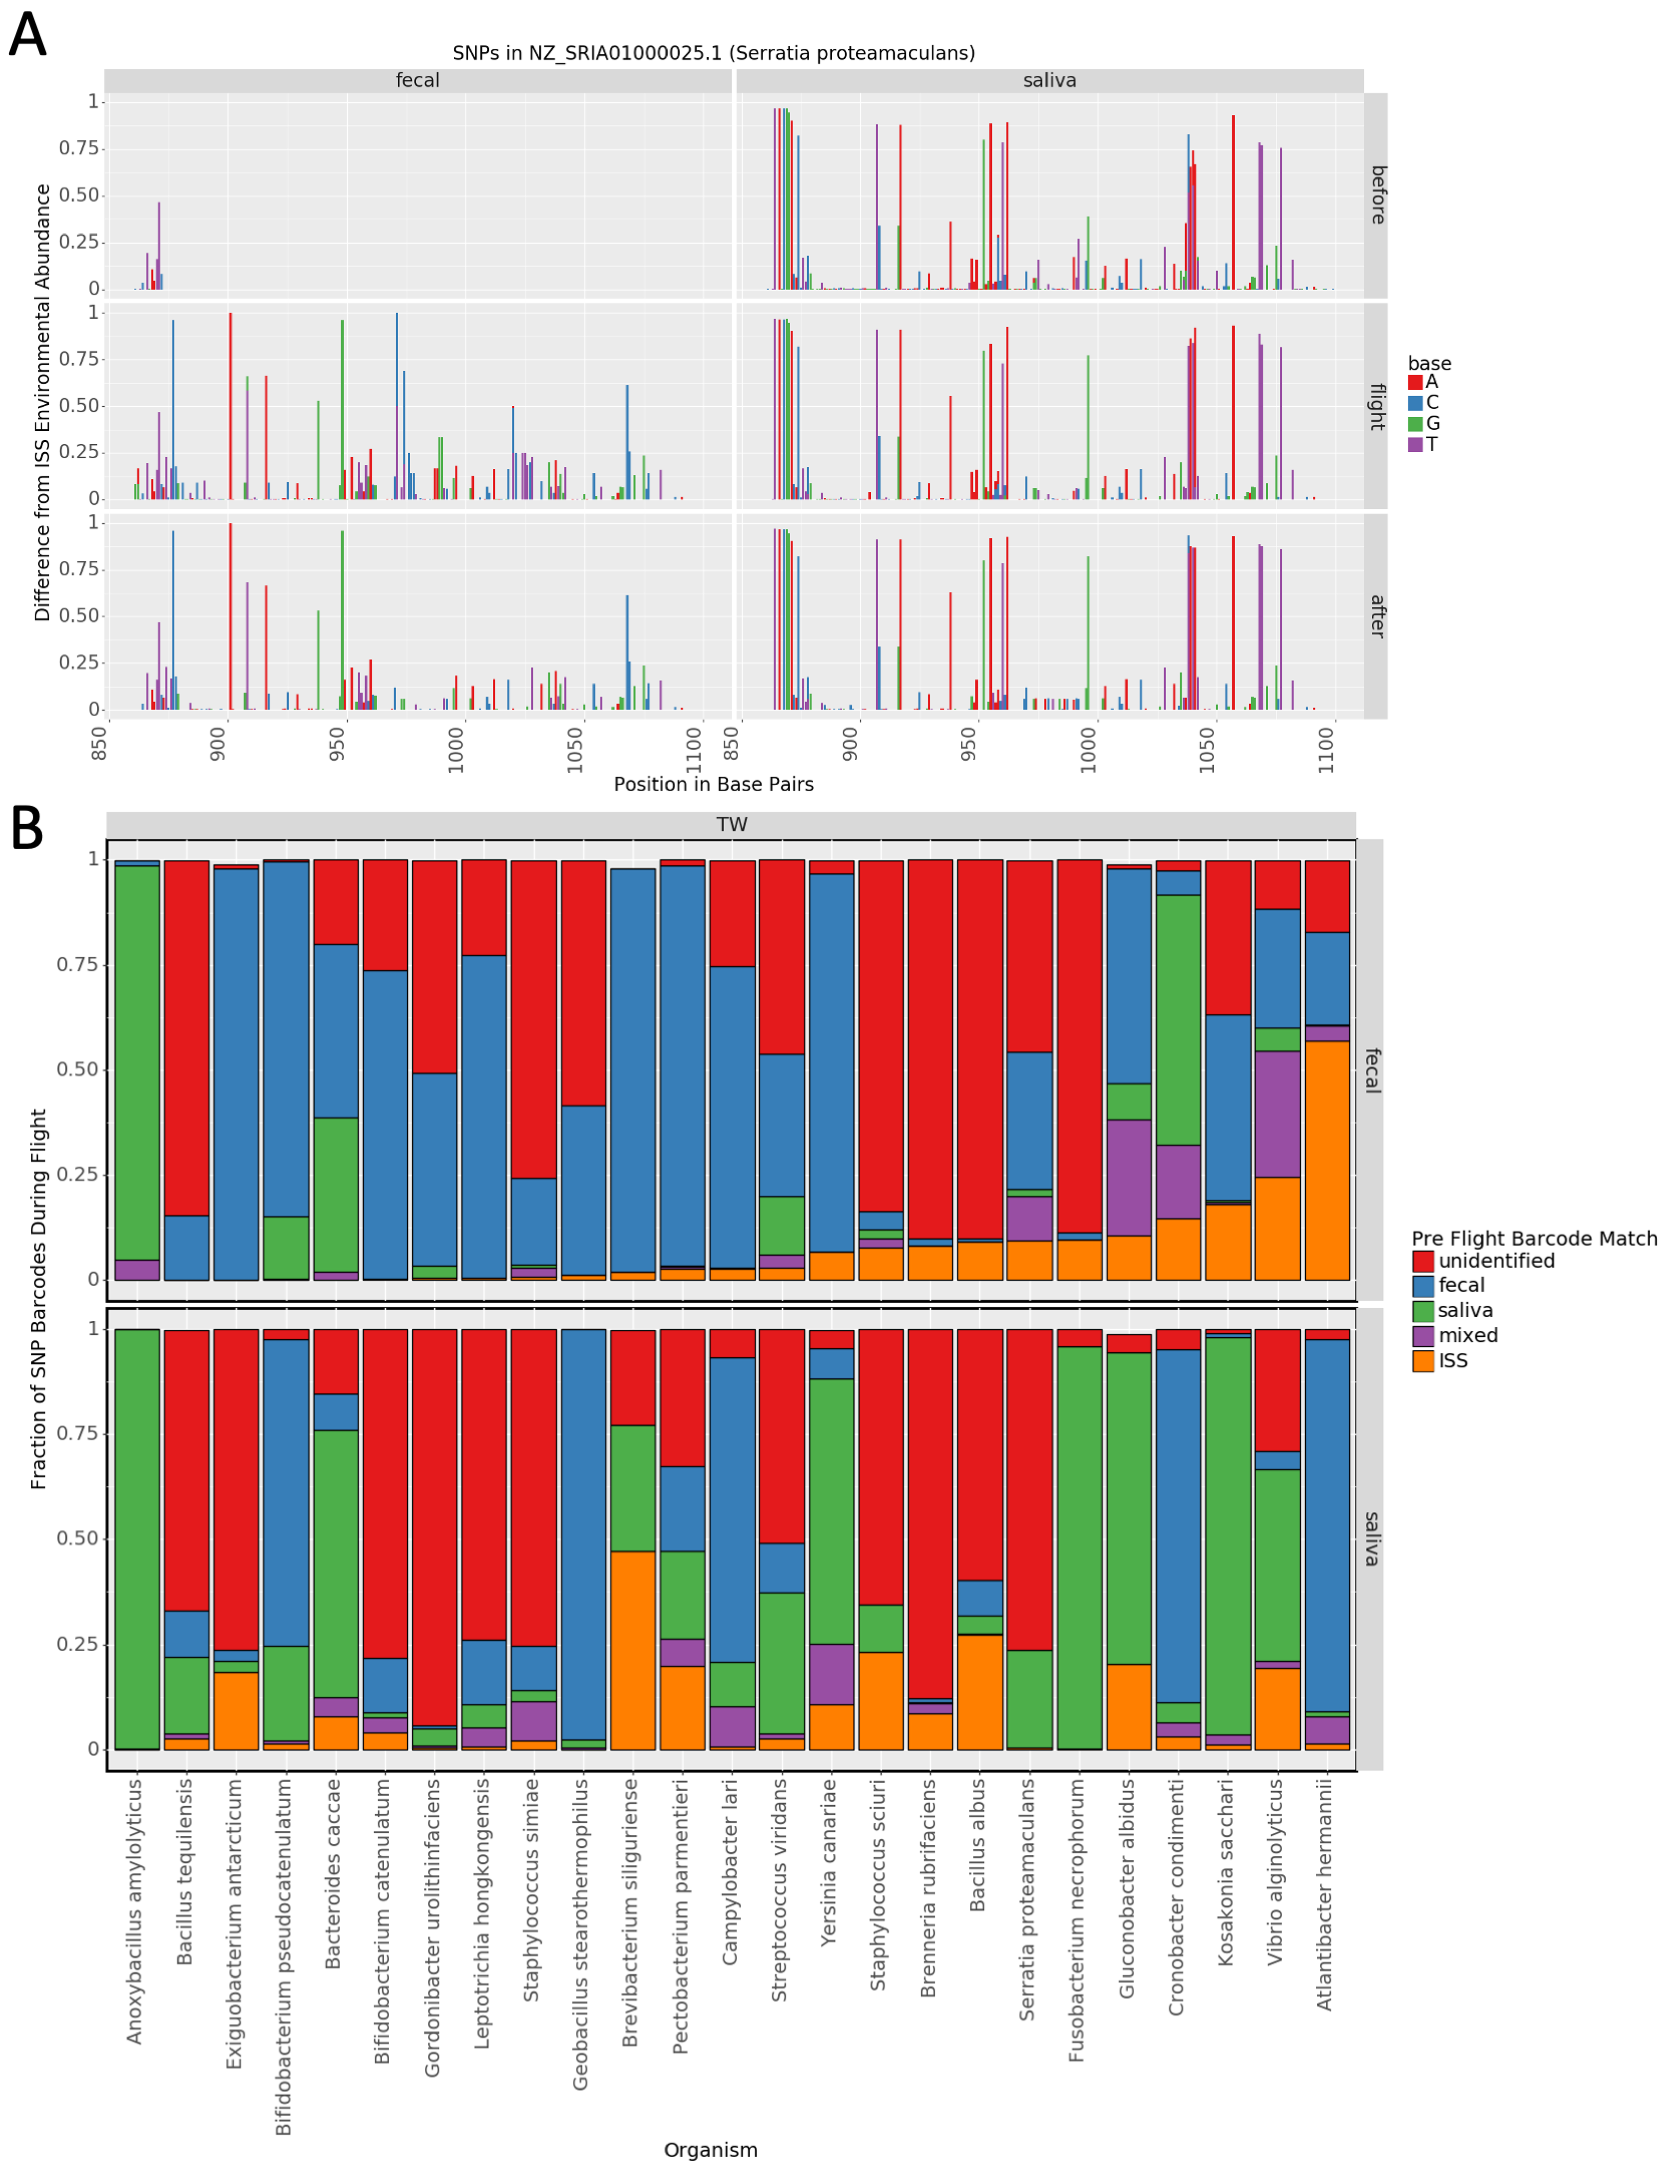
\includegraphics[width=0.99\textwidth]{figs/snp_bcs.png}
%	\vspace{-20pt}
	\caption{\small{
	    A) An example set of SNPs found in Serratia proteamaculans. The abundance of each SNP is shown relative to the frequency of the base found in the ISS at each position. A tall column indicates a base was low abundance in the ISS environment. In this case the SNPs shown for the fecal (left) strain match a secondary strain in the environment and constitute a candidate for transfer from the environment to the gut microbiome.
	    B) Pre-flight sources of different SNP barcodes observed in TW during flight. Each SNP barcode in peri-flight samples from TW was matched to barcodes in pre-flight samples from TW and ISS samples. The fraction of barcodes matching each source is shown. For fecal samples barcodes labeled as saliva did not match fecal samples and vice versa. Barcodes labeled as matching ISS were not found in either fecal or saliva samples.
	}}
    \label{fig:bcsources}
  \end{center}
%  \vspace{-20pt}
 % \vspace{1pt}
\end{figure}


We identified co-occurring clusters of SNPs in the selected taxa listed above in all samples from TW, HR, and the ISS. We refer to these clusters as SNP barcodes. An example of two such barcodes can be seen in Figure \ref{fig:bcsources}A. We matched SNP barcodes taken in samples taken from TW during flight (concatenated together) to possible sources in pre-flight TW samples and ISS samples. For peri-flight fecal samples we considered four groups: SNP barcodes found in pre-flight fecal samples, barcodes found in pre-flight saliva but not fecal samples, barcodes found in the ISS but neither saliva nor fecal, and barcodes not observed in any other group. Saliva samples were split analogously save that fecal and saliva sources were swapped.

The pre-flight sources of SNP barcodes varied by the species being investigated (Figure \ref{fig:bcsources}B). Some species, such as \textit{Cronobacter condimenti} showed an apparent flip of strains from the gut microbiome to saliva and vice versa. Other taxa, like \textit{Atlantibacter hermannii}, showed a large fraction of barcodes that matched environmental barcodes in the gut microbiome. Some taxa, like \textit{Bifidocaterium catenulatum} showed little similarity to any potential external source.

Taken together matching regions and SNPs strongly supports the idea that novel taxa in peri-flight commensal microbiomes from TW could come from the environment or from other commensal microbiomes. The size of transferred regions and number of SNPs suggests that taxa transfer between commensal microbiomes more frequently than they transfer from the environment to commensal microbiomes. However, these rates may prove to be anomalous for either TW, habitation in the ISS, or both.
